\documentclass{article}

% Packages for code, figures, and automata
\usepackage{listings} % For code listings
\usepackage{graphicx} % For including figures
\usepackage{tikz}     % For drawing automata
\usepackage{multirow}
\usepackage{array}
\usepackage{amssymb} % Pacchetto per simboli matematici
\usepackage{float}
\usepackage{nicematrix}
% \usepackage[style=numeric-comp,useprefix,hyperref,backend=bibtex]{biblatex}

\usepackage{pgfplots}
\usepackage{amsmath}


%colorize lstlisting with language
\usepackage{xcolor}
\usepackage{titlesec}
\usepackage{titlepic}
\usepackage[scaled]{helvet}
\renewcommand\familydefault{\sfdefault}

%import all important packages 

% Packages for code, figures, and automata
\usepackage{listings} % For code listings
\usepackage{graphicx} % For including figures
\usepackage{tikz}     % For drawing automata
\usepackage{multirow}
\usepackage{array}
\usepackage{amssymb} % Pacchetto per simboli matematici
\usepackage{float}

\usepackage{pgfplots}
\usepackage{amsmath}

%colorize lstlisting with language
\usepackage{xcolor}

\usepackage{titlesec}

%package for theorem
\usepackage{amsthm}
\newtheorem*{theorem}{theorem}

%import all important packages 

% Configurazione degli stili per tutti i linguaggi
\lstset{
    basicstyle=\ttfamily,
    keywordstyle=\color{blue},
    commentstyle=\color{purple},
    stringstyle=\color{red},
    % Altre opzioni
    breaklines=true, showstringspaces=false,
    emph={label},
    emphstyle={\color{custompurple}},
    escapeinside={(*}{*)}
    }

% Stile globale per tutti i linguaggi
\lstdefinestyle{mystyle}{
    backgroundcolor=\color{white},
    commentstyle=\color{purple},
    keywordstyle=\color{blue},
    numberstyle=\tiny\color{gray},
    stringstyle=\color{red},
    basicstyle=\ttfamily\footnotesize,
    breakatwhitespace=false,
    breaklines=true,
    captionpos=b,
    keepspaces=true,
    numbers=left,
    numbersep=5pt,
    showspaces=false,
    showstringspaces=false,
    showtabs=false,
    tabsize=2
}

% Impostazioni per tutti i linguaggi
\lstset{style=mystyle}
% Definizione di simboli per subsection e subsubsection
\newcommand{\subsecsymbol}{\textcolor{custompurple}{\rule[0pt]{10pt}{10pt}\hspace{10pt}}}
\newcommand{\subsubsecsymbol}{\textcolor{custompurple}{\textbf{$\blacklozenge$}\hspace{4pt}}}

\titleformat{\section}[block]
  {\Huge\bfseries}
  {\llap{\textcolor{custompurple}{\rule[-4pt]{10pt}{18pt}\hspace{10pt}}\thesection\hskip 12pt}}
  {0pt}
  {}
% Definizione di uno stile per \subsection
\titleformat{\subsection}[block]
  {\Large\bfseries\color{black}}
  {\llap{\subsecsymbol}\thesubsection\hskip 12pt}
  {0pt}
  {}

% Definizione di uno stile per \subsubsection
\titleformat{\subsubsection}[block]
  {\large\bfseries\color{black}}
  {\llap{\subsubsecsymbol}\thesubsubsection\hskip 12pt}
  {0pt}
  {}


%make link clickable
\usepackage{hyperref}
\usepackage{pgfplots}

%use asmath
\usepackage{amsmath}

\usepackage{fancyhdr}
\pagestyle{fancy}
\fancyhf{}
\fancyhead[R]{\nouppercase{\rightmark}}
\fancyfoot[C]{\thepage}

\usepackage{listings}
\usepackage{tabularx}

%color link orange
\hypersetup{
    colorlinks=true,
    linkcolor=custompurple,
    filecolor=magenta,
    urlcolor=cyan,
}

\definecolor{custompurple}{HTML}{8b3fff}

% Define title and author
\begin{titlepage}
    \title{\color{nodeblue}\fontsize{32}{38}\selectfont \textbf{Optimization for Machine Learning - Notes}}  % Change this line
    \author{
        \begin{tabular}{c}
            \textbf{Daniele Avolio - 242423}   \\
        \end{tabular}
    }
    % write academic year
    \date{Academic Year 2023/2024}

\end{titlepage}

\pgfplotsset{compat=1.18}
\begin{document}

\maketitle
\newpage

\tableofcontents
\listoffigures
\newpage

\section{}
\section{Ottimizzazione senza vincoli}


$$
2x_1^3 - 3x_1^2 -6x_1^2x_2 +6x_1x_2^2 +6x_1x_2
$$

Calcoliamo il gradiente e la matrice hessiana

$$
\nabla f(x) = \begin{bmatrix}
6x_1^2 - 6x_1 - 12x_1x_2 + 6x_2^2 + 6x_2 \\
-6x_1^2 + 6x_1^2 + 12x_1x_2 + 6x_1 
\end{bmatrix}
$$

Ora calcoliamo la matrice hessiana

$$
\nabla^2 f(x) = \begin{bmatrix}
12x_1 - 6 - 12x_2 & -12x_1 + 12x_2 + 6 \\
-12x_1 + 12x_2 + 6 & 12x_1
\end{bmatrix}
$$

Spieghiamo i passaggi per il calcolo della Hessiana

$$
\frac{\partial^2 f}{\partial x_1^2} = 12x_1 - 6 - 12x_2
$$

$$
\frac{\partial^2 f}{\partial x_1 \partial x_2} = -12x_1 + 12x_2 + 6
$$

Qui il $-12x_1 + 12x_2 + 6$ viene fuori dal seguente passaggio

In parole povere, prima si calcola la derivata parziale di f rispetto a x1, e poi si calcola la derivata di quel risultato rispetto a x2.
$$
f(x1, x2) = 2x1^3 - 3x1^2x2 + 6x1x2^2 + x2^2 + 6x1x2
$$

$$
= 6x1^2 - 6x1x2 + 6x2^2 + 6x2
$$

$$
= -12x1 + 12x2 + 6
$$


$$
\frac{\partial^2 f}{\partial x_2 \partial x_1} = -12x_1 + 12x_2 + 6
$$

$$
\frac{\partial^2 f}{\partial x_2^2} = 12x_1
$$

Quindi, per spiegare ocme funziona.

Data una funzione, bisogna calcolare inizialmente il \textbf{gradiente}.

Applicando la \textbf{condizione necessaria di primo ordine} troviamo i punti stazionari, ovvero quelli in 
cui il $\nabla f(x) = 0$. Cioé, calcoli il gradiente e lo poni uguale a zero.

Ponendo il gradiente uguale a zero bisogna risolvere il sistema di equazioni per trovare 
i possibili punti stazionari. Una volta trovati, nel nostro esempio erano $4$, 
bisogna esaminare i punti utilizzando la \textbf{condizione sufficiente di secondo ordine} e \textbf{la condizione necessaria di secondo ordine}.

Per farlo, si calcola l'Hessiana della funzione \textbf{in un punto}, per ogni punto. Ricorda bene 
come si calcola l'Hessiana, sopratutto quando compaiono due variabili.

Dopo aver calcolato l'hessiana e sostituito con il punto, 
bisogna \textbf{porre} il determinante della hessiana moltiplicata per l'identità con $\lambda$ uguale a zero.

Calcolando il determinante e ponendolo uguale a zero si risolve l'equazione per trovare gli autovalori $\lambda$. In base 
al segno degli autovalori si può dire il "segno", della matrice. Controllando le 
condizioni necessarie e sufficienti di secondo ordine si può dire se il punto è un minimo locale, minimo locale stretto, massimo locale, massimo locale stretto, o punto sella.

\section{Ottimizzazione con vincoli}
In Ottimizzazione con vincoli abbiamo due tipi di vincoli:
\begin{itemize}
    \item Uguaglianza - $g(x) = 0$ - E
    \item Disuguaglianza - $g(x) \geq 0$ - I
\end{itemize}

\textbf{Nota sui programmi quadratici}: Se la funzione obiettivo è del tipo $f(x) = \frac{1}{2}x^TMx+c^Tx$, con $M$ una matrice simmetrica
che significa che $M = M^T$, e tutti i vincoli $g_i$ sono funzioni lineari (sia di Uguaglianza che di Disuguaglianza), allora il problema è un \textbf{programma quadratico}.

Se invece la funzione è $f(x) = c^Tx$, il problema quadratico diventa un programma lineare.

\begin{definition}
    (Vincoli attivo)

    Dato un punto $\bar{x} \in X$, un vincolo $g_i(\bar{x}) = 0$ si dice \textbf{vincolo attivo}.
    
    \textbf{Nota:} Indichiamo $\mathcal{A}(\bar{x})$ l'insieme dei vincoli attivi in $\bar{x}$.
\end{definition}

\subsection{KKT Conditions}
Sono condizioni di ottimalità di primo ordinep per i programmi con vincoli. 

Vediamo in particolare cosa ci interessa:

\begin{definition}
    (LICQ - Linear Independence Constraint Qualification)

    Dato un punto $\bar{x} \in X$, LICQ regge in $\bar{x}$ se l'insieme $\{\nabla g_i(\bar{x}), i \in \mathcal{A}(\bar{x})\}$ 
    cioè l'insieme dei vincoli attivi per $\bar{x}$, deve essere costituito solamente da vettori linearmente indipendenti.
\end{definition}

\begin{definition}
    (Funzione Lagrangiana)

    Dato uno vettore $\lambda \in R^{|E|+|I|}$ chiamato vettore dei moltiplicatori Lagrangiani, diciamo che la funzione lagrangiana di $P$ è:

    $$
    \mathcal{L}(x,\lambda) = f(x) - \sum_{i \in E} \lambda_i g_i(x) - \sum_{i \in I} \lambda_i g_i(x)   
    $$
    con $\lambda \geq 0 \ \forall i \in I$. 
\end{definition}

Se vogliamo fare un esempio, ecco la spiegazione di come si lavora.

Data una regione ammissibile, quindi un insieme di vincoli, analizziamo prendendo un punto $\bar{x}$
come si comportano i vincoli.

Controlliamo quali sono i vincoli che si attivano, ovvero quando la funzione $g_i(\bar{x}) = 0$.

Prendiamo questi vincoli e calcoliamo il gradiente del vincolo, ovvero $\nabla g_i(\bar{x})$.
Se abbiamo ancora delle variabili dopo aver fatto il gradiente, sostituiamo alla $x$ che 
compare nel gradiente il punto $\bar{x}$.

Poi, dopo aver calcolato questi valori, inseriamo tutti i gradienti in una matrice, chiamata $B$. 
Bisogna controllare che i gradienti siano linearmente indipendenti, e per comodità
possiamo calcolare il \textbf{determinante} della matrice e controllare che sia $\neq 0$.

Se ad occhio si vede che dei gradienti sono linearmente dipendenti, allora si può dire 
direttamente che $LICQ$ non reggono.


\section{Approcci di classificazione}
\label{sec:approcci-di-classificazione}

Abbiamo diversi approcci di classificazione.

\begin{itemize}
    \item \textbf{Supervised learning}: Abbiamo un'insieme di dati che sono \textbf{etichettati}.
          Questo rappresenta il nostro \textbf{training set}. Il nostro obiettivo è fare
          predizioni sulle etichette di dati non ancora visti. Le etichette rappresentano
          la \textbf{classe}.
    \item \textbf{Unsupervised Learning}: I dati non hanno alcuna etichetta. Il nostro
          obiettivo è fare operazioni di \textbf{clustering}, ovvero raggruppare i dati in base a quanto sono simili tra loro.
    \item \textbf{Semisupervised Learning}: Abbiamo entrambi i tipi di dati (con e senza etichette). L'obiettivo è predirre la label
          dei dati non etichettati.
\end{itemize}

Il modo in cui chiamo i dati all'interno del nostro dataset sono molteplici,
tipo:
\begin{enumerate}
    \item Datum
    \item Object
    \item Feature Vectore / Vettore delle caratteristiche
    \item Punto
\end{enumerate}

\begin{definition}
    (Classifier)

    Un classificatore è una \textbf{superficie di separazione} tra le classi.
\end{definition}
\newpage
\section{Separazione Lineare}
\begin{definition}
    (Separazione Lineare)
    Dati due insiemi $A = \{a_1, a_2, \dots, \_m\}$ e $B = \{b_1, b_2, \dots, b_k\}$. Due insiemi si dicono \textbf{linearmente separabili} $\iff$ esiste un iperpiano $H(v,\gamma)$ che separa i due insiemi.

    $$
        H(v,\gamma) = \{x \in \mathcal{R}^n | v^T x = \gamma\}
    $$
    con:
    \begin{itemize}
        \item $v \in R^n$ è un vettore, la normale del piano
        \item $\gamma \in R$ è uno scalare, il bias
        \item $v \neq 0$
    \end{itemize}

    Questo iperpiano, tale che:

    $$
        v^T a_i \geq \gamma + 1 \land v^T b_j \leq \gamma - 1
    $$
    per $i = 1, \dots, m$ e $j = 1, \dots, k$.
\end{definition}

\textbf{Nota e possibile domanda}: Quando andiamo a classificare non teniamo conto del +1 e -1, perché vengono usati solo per costruzione.
Quindi la disequazione conta solamente il valore di $\gamma$ (nel lato desto).

\textbf{Nota 2:} I due insiemi $A$ e $B$ sono linearmente separabili $\iff$ \textbf{l'intersezione} della loro copertura convessa è vuota.
$$
    conv(A) \cap conv(B) = \emptyset
$$

\begin{definition}
    (Copertura Convessa)

    La copertura convessa di un'insieme $X$ è l'insieme convesso più piccolo che lo
    contiene.

    Un'insieme si dice convesso se per ogni coppia di punti $(x,y) \in X$ la
    combinazione di $x$ e $y$ è sempre all'interno dell'insieme $X$. Formalmente:
    $$ \forall x,y \in X, \forall \lambda \in [0,1] \implies \lambda x + (1 -
        \lambda) y \in X $$
\end{definition}

Implicazione ovvia, ma la copertura convessa di un'insieme convesso è l'insieme
stesso. $ X\ convesso \implies conv(X) = X $

\begin{definition}
    (Funzione Errore | Loss Function)

    Un punto $a_i \in A$ è \textbf{classificato correttamente} se $$ v^T a_i \geq
        \gamma + 1 \implies v^T a_i - \gamma - 1 \geq 0 $$ Questo implica che $a_i$ è
    \textbf{classificato erroneamente} se $$ v^T a_i - \gamma -1 < 0 \implies -v^T
        a_i + \gamma + 1 > 0 $$

    L'errore di $a_i$ è dato da: $$ \max\{0, -v^T a_i + \gamma + 1\} \geq 0 $$

    Analogamente, un punto $b_j \in B$ è \textbf{classificato correttamente} se $$
        v^T b_j - \gamma + 1 \leq 0 $$. Questo implica che $b_j$ è \textbf{classificato
        erroneamente} se $$ v^T b_j - \gamma + 1 > 0 $$

    L'errore di $b_j$ è dato da: $$ \max\{0, v^T b_j - \gamma + 1\} \geq 0 $$

    La funzione errore totale che ci viene da: $min_{v,\gamma} f(v,\gamma)$ è:

    $$
    \min_{v,\gamma} f(v,\gamma) = \frac{1}{m} \sum_{i=1}^{m} \max\{0, -v^T a_i + \gamma + 1\} + \frac{1}{k} \sum_{j=1}^{k} \max\{0, v^T b_j - \gamma + 1\}
    $$

    Cioè, la media degli errori di classificazione dei punti di $A$ e $B$.

    Questa funzioen è \textbf{non smooth e convessa}. Possiamo trasformare questo in un programma lineare.

    Consideriamo:
    \begin{itemize}
        \item $\xi  = \max{0, -v^T a_i + \gamma + 1}$ per $i = 1, \dots, m$
        \item $\psi_j = \max{0, v^T b_j - \gamma + 1}$ per $j = 1, \dots, k$
    \end{itemize}

    Possiamo riscrivere il problema nel seguente modo:

    $$
    LP = \begin{cases}
        \min_{v,\gamma, \xi, \psi} \frac{1}{m} \sum_{i=1}^{m} \xi_i + \frac{1}{k} \sum_{j=1}^{k} \psi_j \\

        \xi_i \geq -v^T a_i + \gamma + 1 \quad \forall i = 1, \dots, m \\
        \psi_j \geq v^T b_j - \gamma + 1 \quad \forall j = 1, \dots, k \\
        \xi_i, \psi_i \geq 0 \quad \forall i = 1\\
    \end{cases}
    $$
\end{definition}

\section{Separazione Poliedrale}
La separazione poliedrale è un'estensione della separazione lineare. In questo caso
consideriamo un problema che ha almeno $h > 1$ iperpiani di separazione $H(v^j, \gamma_j)$ tale che:
\begin{enumerate}
    \item Per ogni punto positivo $a_i \in A$ e ogni iperpiano $j = 1, \dots, h$ vale che:
    $$
        v^{jT} a_i \geq \gamma_j - 1
    $$

    Cioé il punto è "dentro" l'iperpiano.

    \item Per ogni punto negativo $b_i \in B$ esiste almeno 1 iperpiano $j \in \{1, \dots, h\}$ tale che:
    $$
        v^{jT} b_i \geq \gamma_j + 1
    $$

    Cioé il punto è "fuori" almeno 1 iperpiano.
\end{enumerate}

\textbf{Nota:} $A$ è h-pliedricamente separabile da $B$ $\iff$ $conv(A) \cap B = \emptyset$.

\textbf{Nota 2:} Se h = 1 $\rightarrow$ problema lineare.

\begin{definition}
    Funzione errore nel caso poliedrico:

    Un punto $a_i \in A$ è classificato correttamente se:

    $$
        v^{jT} a_i \leq \gamma_j -1 \quad \forall j = 1, \dots, h
    $$

    $$
        v^{jT} a_i - \gamma_j + 1 \leq 0 \quad \forall j = 1, \dots, h
    $$

    $$
        \max_{j=1, \dots, h} \{v^{jT} a_i - \gamma_j + 1\} \leq 0 \quad \forall j = 1, \dots, h
    $$

    Ed è classificato erroneamente se:

    $$
    \max_{j=1, \dots, h} \{v^{jT} a_i - \gamma_j + 1\} > 0 \quad \forall j = 1, \dots, h
    $$

    In totale, l'errore di $a_i$ è dato da:

    $$
        \max_{j=1, \dots, h} \{0, v^{jT} a_i - \gamma_j + 1\}
    $$

    Per quanto riguarda i punti negativi $b_j \in B$, viene classificato 
    correttamente se $\exists j \in \{1, \dots, h\}$ tale che:

    $$
    v^{jT} b_i \geq \gamma_j + 1 \rightarrow v^{jT} b_i - \gamma_j - 1 \geq 0 \rightarrow -v^{jT} b_i + \gamma_j + 1 \leq 0
    $$

    Analogamente, viene classificato erroneamente se:

    $$
    -v^{jT} b_i + \gamma_j + 1 > 0 \quad \forall j = 1, \dots, h
    $$

    Cioè, se $\min_{j=1, \dots, h} \{-v^{jT} b_i + \gamma_j + 1\} > 0$.

    L'errore di $b_i$ è dato da:

    $$
    \max_{j=1, \dots, h} \{0, -v^{jT} b_i + \gamma_j + 1\}
    $$    

    Notiamo che questa funzione è \textbf{più difficile da minimizzare}.

    \begin{figure}[H]
        \centering
        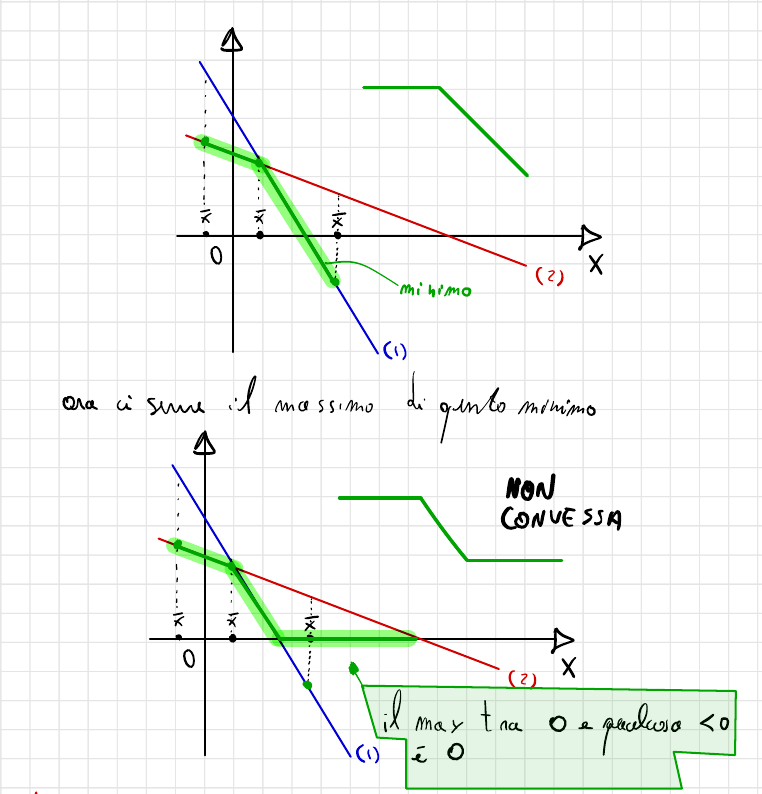
\includegraphics[width=0.8\linewidth]{images/tosta.png}
        \caption{Funzione di errore nel caso poliedrico}
        \label{fig:3-1}
    \end{figure}
    
    La funzione di errore 
    totale è data da:

    $$
        f ( v^1, v^2, \dots, v^; \gamma_1, \gamma_2, \dots, \gamma_h ) = \frac{1}{m} \sum_{i=1}^{m} \max_{j=1, \dots, h} \{0, v^{jT} a_i - \gamma_j + 1\} + \frac{1}{k} \sum_{j=1}^{k} \max_{j=1, \dots, h} \{0, -v^{jT} b_i + \gamma_j + 1\}
    $$

    Questa funzione è \textbf{non convessa}.
\end{definition}


\section{Separazione Sferica}



\bibliographystyle{plain}
\bibliography{references}  % if your .bib file is named references.bib
\end{document}